\subsection{Performance Metrics and Benchmarks}
A computer user focuses on minimizing \textbf{response time} (or \textbf{execution time}), while a warehouse-scale operator aims to maximize \textbf{throughput}, the total work completed in a given period.\sidenote{John L. Hennessy and David A. Patterson,
	\textit{Computer Architecture: A Quantitative Approach},
	5th ed., Morgan Kaufmann, 2011.}

We want to relate the performance of two different computers, say, $X$ and $Y$. For the phase \begin{center}
``$X$ is faster than $Y$'',
\end{center} we can define it in terms of execution times: let
\begin{itemize}
	\item \( T_X \) denote the execution time of computer \( X \),
	\item \( T_Y \) denote the execution time of computer \( Y \).
\end{itemize} If \( X \) is faster than \( Y \), then:
\[
T_X < T_Y
\]
This inequality means that the time required for \( X \) to complete the task is less than the time required for \( Y \).

In particular, ``$X$ is $n$ times faster than $Y$''\sidenote{
The computer $X$ is 1.5 times faster than $Y$ means that \[
1.5=\frac{\text{Execution Time}_Y}{\text{Execution Time}_X}.
\] If $\text{Execution Time}_X=10$s and $\text{Execution Time}_Y=15$s, TFAE:
\begin{itemize}
	\item $X$ is 1.5 times faster than $Y$
	\item $Y$ is about 0.76 times slower than $X$.
\end{itemize}
} means that \[
\frac{\text{Execution Time}_Y}{\text{Execution Time}_X}=n.
\] Since execution time is the reciprocal of performance, the following relationship holds:
\[
n = \frac{\text{Execution Time}_Y}{\text{Execution Time}_X} =\frac{\displaystyle 1/\text{Performance}_Y}{\displaystyle 1/\text{Performance}_X}= \frac{\text{Performance}_X}{\text{Performance}_Y}.
\]
where: \begin{itemize}
	\item \( n > 1 \): Computer \( X \) is \( n \) times faster than \( Y \).
	\item \( n < 1 \): Computer \( X \) is \( 1/n\) times slower than \( Y\). In other words, computer $Y$ is $1/n$ times faster than computer $X$.
\end{itemize} 

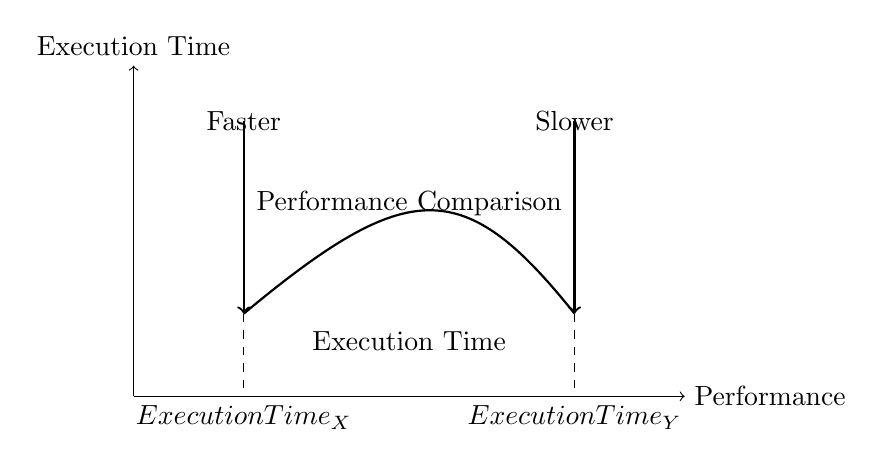
\begin{tikzpicture}[scale=0.7]
	\draw[->] (0,0) -- (10,0) node[right] {Performance};
	\draw[->] (0,0) -- (0,6) node[above] {Execution Time};
	
	\node[align=center] at (2,5) {Faster};
	\node[align=center] at (8,5) {Slower};
	
	\draw[thick, ->] (2,5) -- (2,1.5);
	\draw[thick, ->] (8,5) -- (8,1.5);
	
	% Dotted line for Execution Time X
	\draw[dashed] (2,1.5) -- (2,0) node[below] {$\text{Execution Time}_X$};
	\draw[dashed] (8,1.5) -- (8,0) node[below] {$\text{Execution Time}_Y$};
	
	% Execution Time labels
	\node[align=center] at (5,1) {Execution Time};
	
	% Performance Curve
	\draw[thick] (2,1.5) .. controls (5,4) and (6,4) .. (8,1.5);
	
	% Performance Label
	\node[align=center] at (5,3.5) {Performance Comparison};
\end{tikzpicture}